\begin{figure}[H]
\centering
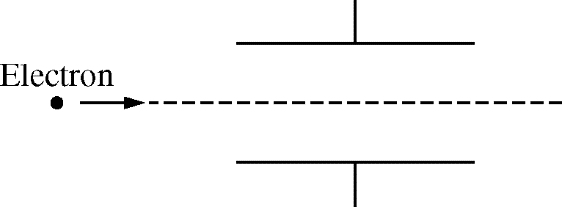
\includegraphics[scale=0.4]{images/img-013-029.png}
\end{figure}

% Multiple Choice Question 31
\begin{questions}\setcounter{question}{30}\question
Uniform magnetic and electric fields exist between the two oppositely charged parallel plates shown in the figure above. An electron travels horizontally between the plates. Assuming gravitational effects to be negligible, which of the following diagrams shows a combination of electric and magnetic field directions that will allow the electron to travel undeflected?

\begin{oneparchoices}
\choice \adjustbox{valign=t}{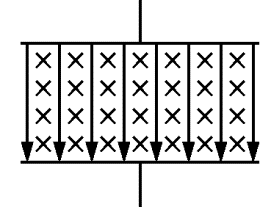
\includegraphics[scale=0.4]{images/img-013-030.png}}
\choice \adjustbox{valign=t}{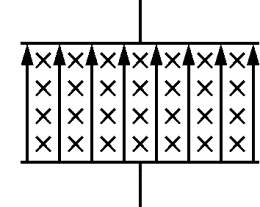
\includegraphics[scale=0.4]{images/img-013-031.png}}
\choice \adjustbox{valign=t}{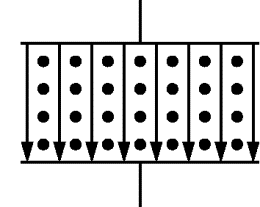
\includegraphics[scale=0.4]{images/img-013-032.png}}
\choice \adjustbox{valign=t}{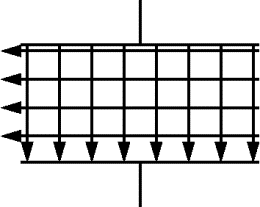
\includegraphics[scale=0.4]{images/img-013-033.png}}
\choice \adjustbox{valign=t}{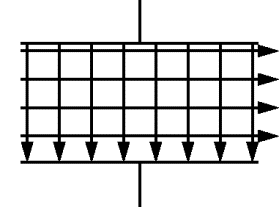
\includegraphics[scale=0.4]{images/img-013-034.png}}
\end{oneparchoices}\end{questions}

